%Template credit: Jan-Willem Steeb, NRAO

\documentclass[12pt,a4paper]{article}

\usepackage{graphics,graphicx}
\usepackage[%
    font={small,sf},
    labelfont=bf,
    format=hang,    
    format=plain,
    margin=0pt,
    width=0.8\textwidth,
]{caption}
\usepackage[list=true]{subcaption}
\usepackage{amsmath}
\usepackage{amssymb}
\usepackage{bm}
\usepackage{listings}
\usepackage{hyperref}
\usepackage{lmodern}  
\usepackage{amsmath}  
\usepackage{xcolor}
% PJT
\usepackage{enumitem}
%\usepackage{times}
%\usepackage{mathptmx}


\lstset{
  basicstyle=\ttfamily,
  columns=fullflexible,
  frame=single,
  breaklines=true,
  postbreak=\mbox{\textcolor{red}{$\hookrightarrow$}\space},
}

\textheight=247mm
\textwidth=180mm
\topmargin=-7mm
\oddsidemargin=-10mm
\evensidemargin=-10mm
\parindent 10pt

%%%%%%%%%%%%%%%%%%%%%
%%%%% Custom Commands %%%%
%%%%%%%%%%%%%%%%%%%%%
\newcommand{\vb}[1]{\text{\textbf{#1}}} %make non special characters bold in math mode, used for vectors and matrices
\newcommand{\n}[1]{\text{{#1}}} %removes math styling, useful for subscripts

%Mathematic Functions
\DeclareMathOperator*{\argmax}{arg\,max}
\DeclareMathOperator*{\argmin}{arg\,min}
\DeclareMathOperator*{\mmid}{mid}
\DeclareMathOperator*{\at}{arctan2}

%%%%%%%%%%%%%%%%%%%%%
%%%%% Start of document %%%%% 
%%%%%%%%%%%%%%%%%%%%%

\begin{document}
\pagestyle{plain}
\pagenumbering{arabic}
 
%%%%%%%%%%%%%
%%%%% Title  %%%%%
%%%%%%%%%%%%%%

\begin{center}
{\Large{\bf{  GBO stuff  \\  }}} 

\end{center}
\bigskip

\centerline{Peter Teuben (University of Maryland, USA)}

\centerline{Version 0.5 - \today}
\bigskip

\begin{abstract}

This is a working document discussing the status of SD data analysis
systems, focusing on updating the GBO system with a modern python3
based eco-system. Supporting code and documentation can be found in
\url{https://github.com/teuben/gbtoy}.

\end{abstract}

\section{Introduction for non-SD users}

Here we discuss a Single Dish (SD) data analysis package.  SD data are
much easier to understand than most other astronomical formats,
yet they can exhibit as much complexity as associated with other formats.

On the top level they are just a ``collection'' of spectra, where a
spectrum is a 1-dimensional array\footnote{for Parkes spectra
  of length N are viewed multi-dimensional, and
  become (N/2, 2, 1, 1), where the 2nd dimension is STOKES.   However, GBO
  always stores them as (N,1,1,1) where STOKES is the 4th and last axis,
  and designated via CTYPE4}. Each spectrum has meta-data that describe
where and how the data was taken. Of course position on sky and
frequency setting, but another 40-80 extra variables are not uncommon.
Although there is a standard for this, many variables wind up to be telescope
specific. In the past a simple stack based spectrum calculator was the
basic data analysis system for SD data.
Even more modern systems are essentially still of this nature.
 
For a collection of spectra that cover an area of the sky (the modern
term is ``On-The-Fly'' (OTF) mapping), another step can be taken after
the spectra have been calibrated, and that is gridding and mapping
(imaging) these spectra into an image cube.

\begin{figure}[h]
\centering
  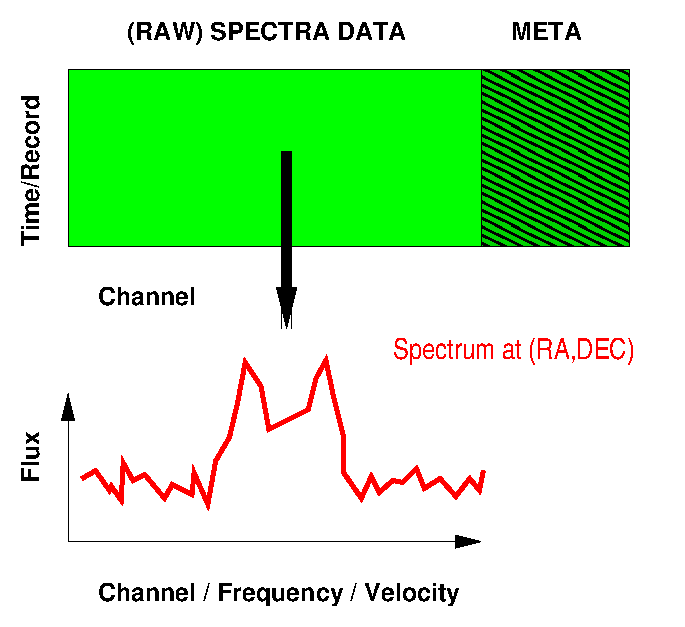
\includegraphics[width=0.4\textwidth]{fig2.eps}
  \caption{\label{bintable} SDFITS BINTABLE: spectra data and meta-data.
    Typically different rows in the DATA are manipulated (ON/OFF and averaging)
    to result in a final single spectrum for a given RA/DEC. See also
    figure \ref{waterfall}.}
\end{figure}


\section{Overview}

The GBT/GBO\footnote{you will see a lot of documentation using GBT and
  GBO interspersed} single dish processing software is reviewed in
light of a more coherent workflow using python on the top level, and
abandoning the IDL licensed software.\footnote{weather info is also
  needed in some calibration procedures, making it still hard to work
  offsite}

The current data format is SDFITS, and will continue to be used, as
this is an astronomy wide industry standard, as well as a lot of
investment of tools at GBO that write SDFITS files. Most of the raw
data before it turns into SDFITS are actually also FITS tables, which
are standardized at the GBO, but they will not concern on in this
paper.

We will however take this opportunity to review the whole workflow of
SD data processing from the astronomers' point of view, by
comparing functionality offered in other packages such as {\tt comb},
{\tt SPECX}, and {\tt CLASS}. The predecessors of {\tt GBTIDL} are
{\tt DISH} (under AIPS++) and before that {\tt uniPOPS}. They are
largely functionally equivalent, just using other command
processors. At the current time (2019 as we write this), python is the
most likely candidate for a data processing package dealing with
single dish data. Given popular usage of astropy and jupyter
notebooks, it would also be nice if any new efforts could make use of
this.

\section{Functionality}

What is the functionality we would want from a SD data reduction
package? Very briefly here are some items:


\subsection{Functionality needed for a single spectrum}

\begin{enumerate}

\item Flux/temperature Calibrate: 
  \begin{itemize}
    \item[{\bf a.}]
    simple single value for entire spectrum or array with one 
       value per channel.
    \item[{\bf b.}]
   save calibration array for inspection
    
  \end{itemize}

\item Calculate on-off and nodding spectrum:
  \begin{itemize}
  \item[{\bf a.}]
    on and off spectrum for a single position
  \item[{\bf b.}]   
    on spectrum and a shared off position
  \item[{\bf c.}]   
    on spectrum and a series of off position observations
    averaged to make the off for subtraction
  \item[{\bf d.}]   
    scan map where off positions are determined from
    portions of map with no line signal and averaged
  \item[{\bf e.}]   
    save on and off for inspection
  \end{itemize}

\item   Calculate freq switched spectrum:
  \begin{itemize}
  \item[{\bf a.}]   
    FS spectrum based on single position
  \item[{\bf b.}]   
    FS spectrum based on reference offset frequency spectrum
  \item[{\bf c.}]   
    save sig and ref freq spectrum for inspection
  \end{itemize}

\item   Fixed noise spectrum:
   Since the spectrum is made by a digital correlator, is there
      a fixed noise pattern that may be constant for hours or days
      that should be calibrated out of all data?
    Is this done before the SDFITs stage?

\item    Baseline removal:
   Set window for channels to be used for baseline calculation
   \begin{itemize}
  \item[{\bf a.}]   
    polynomial fit up to 5th order
  \item[{\bf b.}]   
    sine fit
  \item[{\bf c.}]   
    fourier filter with upper limit specified in channels
  \item[{\bf d.}]   
    option to plot fit on data before removal
  \item[{\bf e.}]   
    should allow for multiple applications
  \item[{\bf f.}]   
   keep array of cumulative removed baseline?
  \end{itemize}

\item RFI removal:
  \begin{itemize}
  \item[{\bf a.}]  
   to be done from rawest data likely based on presence of narrow 
   frequency spike or rms variation over time
  \item[{\bf b.}]  
    could experiment in lag space
  \item[{\bf c.}]      
   replace affected channels with interpolation or NANs
  \end{itemize}

\item Smooth spectra:
  \begin{itemize}
  \item[{\bf a.}]  
    Hanning with optional channel elimination
  \item[{\bf b.}]  
    boxcar summing
  \item[{\bf c.}]
    gaussian
  \item[{\bf d.}]   
   allow for NANs to be replace with values if there
       are actual values within smoothing range.
  \end{itemize}

\item Line parameters:
  \begin{itemize}
  \item[{\bf a.}]
   allow for range of channels for doing calculation
  \item[{\bf b.}]
   calculate mean amplitude, velocity, and integrated
        amplitude -- like moment maps
  \item[{\bf c.}]
   fit gaussian line(s)
  \item[{\bf d.}]
   fit gaussians to lines with hyperfine structure to get
           single mean velocity and width
  \item[{\bf e.}]
   fit the busy function (ascl.net/1402.015) , or via a plugin, any functional shape
  \item[{\bf f.}]
   save line parameters in some way that they can be
           accessed and output for a group of sources or
	   positions
  \end{itemize}

\item Reassign rest frequency:
  \begin{itemize}
  \item[{\bf a.}]   
   assign or reassign rest frequency for observed line
  \item[{\bf b.}]   
   allow for multiple rest frequencies for multiple line
             in spectrum -- alternately allow spectra to
	     be cut into sub-spectra. Allow for sub-windows
	     in spectrum each with a rest freq?
  \end{itemize}

  
\end{enumerate}


\subsection{Functionality needed for collections of spectra}

\begin{itemize}

\item Deal with spectra on an individual (or group) basis [see above]
  \begin{itemize}
  \item Visualize spectra, a versatile interactive plotting tool is needed
  that can handle overlaying fits and/or other spectra
  \item Calibrate spectra (Freq, Pos, Nod, ...)
  \item Flagging/Masking data
  \item Co-adding
  \item Baseline fitting and subtracting
  \item Smoothing, Rebinning
  \item Edit header (e.g. hack to fix problems)  
  \item Fit models to spectra
  \end{itemize}

\item Good batch system for pipeline and/or scripts to define a workflow on one spectrum
  and then apply it to all
  
\item Organize spectra by properties such as RA, DEC (for gridding,
  but also to select what to work on. E.g. a much liked feature of
  CLASS is it ability to select spectra from a database. Make sure we
  can do incrementally do this

\item Gridding spectra in RA,DEC or GLAT,GLON, even in AZ,EL for debugging?

\item Does OTF have special needs?

\item Line and Continuum data have different needs?

\item Keep provenance in SDFITS files

\item Example files with a regression test  

\item integrate well with a python eco-system. Many users are now familiar with
  python, numpy etc.  If the code allows us to get and set numpy arrays,
  that's a gain. It should also be usable via a the classic ``import''
  mechanism, and expected to work well with packages such as astropy and jupyter
  notebooks. Use of widgets would be interesting too, but that's very notebook
  specific.
\end{itemize}

\begin{figure}[h]
\centering
  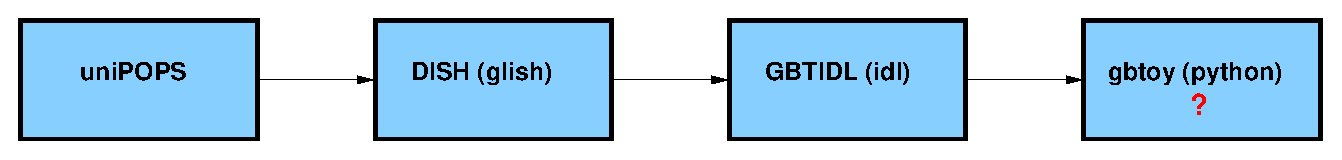
\includegraphics[width=\textwidth]{fig1.eps}
\caption{\label{evolution} Evolution of the GBT analysis software?}
\end{figure}


\section{Existing GBT code}

We are faced with 3 existing packages: {\tt GBTIDL}, {\tt gbt-pipeline} and
{\tt gbtgridder}, of which the latter two are in python2. There is also
a derived product, {\tt gbtpipe}, written by Erik Rosolowsky. All codes are
publicly available. Some code overlap has been noticed in {\tt gbtpipe}.
The pulsar timing observations are
in a completely different category, and will be ``ignored'' for the
moment. Another point to keep in mind is that
the ``dialects'' that seem to exist in the SDFITS format are specific to the instrument.

\bigskip\noindent
{\bf Nomenclature:} of SD observations ({\it as found in some of the GBT documentation}):
    

\begin{itemize}[leftmargin=1in]
  \item[{\bf region}]  : over many days and possibly RA/DEC
  \item[{\bf session}] : same 'day' continguous in time
  \item[{\bf block}]   : observation unit, typically in one SDFITS file (or related SDFITS files with VEGAS)
  \item[{\bf scan}]    : integrations that belong together (few mins)
  \item[{\bf integration}] : integration of a specific state (pointing, band, polarizations, ...)
  \item[{\bf phases}]    : the individual rows in SDFITS that make a specific integration.  In GBTIDL they are also
    referred to as a ``record''.
\end{itemize}   


In addition there are several ways how to calibrate SD spectra, broadly separated
into position and frequency switching. Calibration also depends on the instrument used,
and the SDFITS ``dialect'' will play a role in this.

\begin{itemize}
\item
  {\bf Need updated and better description of the following items, there should be 5 for GBT:}
\item
nodding:    a mirror like device make it look at a different "blank" sky
nodding secondary. or are there other nodding options?
\item
position:   telescope physically looks at a different "blank" sky?
\item
frequency:  use a nearby part of spectrum to be able to baseline subtract
\end{itemize}

OTF (e.g. \cite{2007AA...474..679M})
would scan over the source far enough out that the ``off'' positions are reached at
the edges of the scans, but there are other observing modes possible. GBTIDL is able to
handle a number of standard observing modes, but there there are many non-standard
observing modes that take effort to calibrate with GBTIDL.  Any new system needs to
be flexible to deal with non-standard observing modes.

\section{GBTIDL}

As a reminder, here is an example\footnote{taken from the GBTIDL Users' Guide}
where you get a quick look and feel of the command line interface in GBTIDL:

\begin{lstlisting}[language=bash]
% gbtidl                         # Start GBTIDL from the unix prompt
GBTIDL -> filein, 'myraw.fits'   ; open an SDFITS file
GBTIDL -> summary                ; summary
GBTIDL -> getfs, 9               ; get scan 9 freq. switched spectrum
GBTIDL -> setregion              ; Set region used to determine baseline (interactive)
GBTIDL -> nfit,2                 ; Specify that a 2nd order baseline will be used
GBTIDL -> baseline               ; Fit and subtract a baseline
GBTIDL -> fitgauss               ; Fit a Gaussian profile to the plotted spectrum.
GBTIDL -> stats                  ; show statistics for the spectrum
GBTIDL -> print_ps               ; Write the current spectrum to a postscript file
GBTIDL -> fileout, 'mydata.fits' ; Specify the output file name for saved data
GBTIDL -> keep                   ; Save the spectrum currently displayed
GBTIDL -> exit                   ; Exit GBTIDL

\end{lstlisting}

\begin{figure}[h]
\centering
  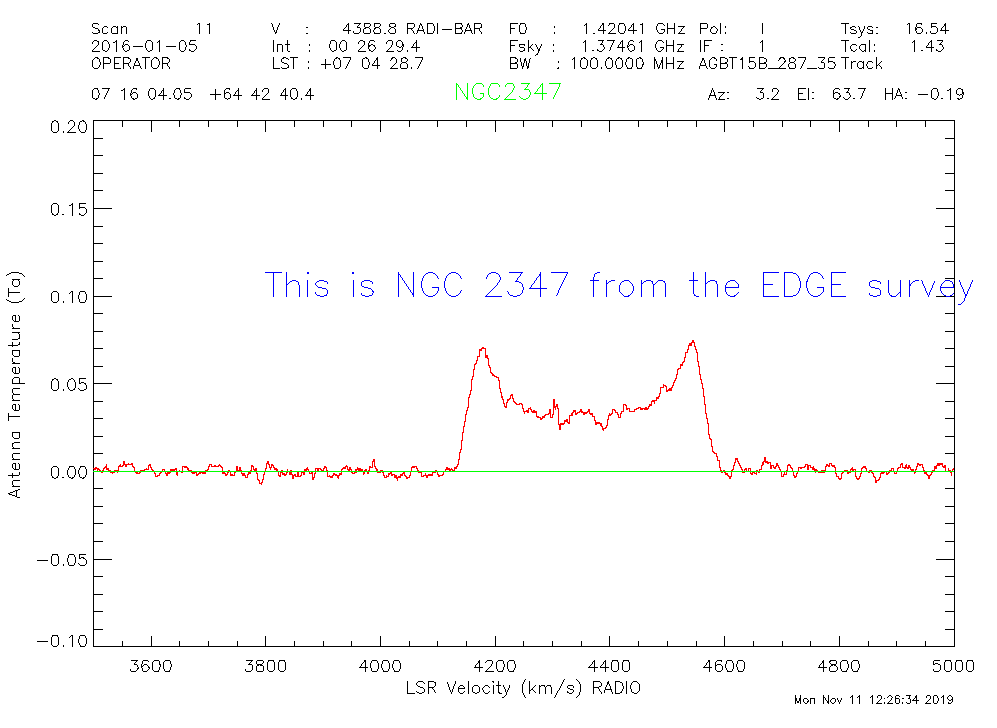
\includegraphics[width=0.75\textwidth]{gbtidl1.png}
\caption{\label{spectrum1} Example GBTIDL spectrum after baseline, not matching the example code!}
\end{figure}


\subsection{Conversion to python?}

GBTIDL can be converted to python in several ways:

\begin{enumerate}
\item
  keep the function names and functionality the same as much as possible,
    but use {\tt pyspeckit} under the hood

\item
  same as 1), but literally  translating IDL to python. A lot more work.
  Functionally the same as  was done uniPOPS to dish to gbtidl it seems.

\item
  using pyspeckit natively. raw python power. This is possibly a harder way for
  existing users to switch to and accept. Might as well force CLASS on them.
  
\item
  bringing the sdfits interfaces that gbt-pipeline uses into the loop.
  probably not useful to 1) , but could be useful for 2)

\item
  alternatively, Astropy's {\tt specutils} infrastructure can also be used
  (specutils, specviz, specreduce) - note that specviz is not in astropy (yet?)

\end{enumerate}

In addition, the peculiar graphics display that GBTIDL is using should
be investigated if pure matplotlib has enough functionality, or do we
need an embedded wxPython ot QtPython interface around it (or another
GUI wrapper).  \url{https://docs.python.org/3/faq/gui.html}
Do we need the Model-View-Controller (MVC) approach, or can we call
matplotlib where needed.

For specutils, the specviz package will need to be investigated, but
should be noted this is not in astropy but still under
spacetelescope.


\section{Data}

\subsection{The SDFITS standard}

Although there is an SDFITS standard, there are some clear dialect
issues. For example, the pyspeckit example file does not work in
GBTIDL. Then, the 3 standard examples from GBTIDL do not work in
pyspeckit, because newer header items (e.g. TRGTLONG) are absent, and
pyspeckit assumes them to be present. They are GBT specific.  The
number of GBT specific header elements has been steadily
increasing. The 2005 data have about 46, there are 79 in the 2016 GBT
EDGE data. The {\tt sdheader} script tries to assembles this knowledge.


\bigskip\noindent

{\bf Nomenclature:} An SDFITS file is a BINTABLE with extension name
``SINGLE DISH''. Each row in the table is a different ``phase'' from
the observation. Each row contains the DATA (the spectrum) and lots of
associated header variables. Since they are in a BINTABLE, they are
called FIELDS (the columns), of which DATA is just one. The other fields
will come in different names: meta-data, header variables, keywords, columns etc.
These are normally varying as function of time, since they are a column in
the BINTABLE. Some SDFITS writers know that a certain column does not change,
and you will find it hidden as a keyword in the FITS header and we sometimes
call those a virtual column. Examples of those are TELESCOP, PROJID, BACKEND,
SITELONG, SITELAT, SITEELEV.

\subsection{Regression testing}

We will need some standard datasets that have known answers. They will need to be in SDFITS format.
A possible contender is an experiment with CLASS formatted files. We currently have in hand,
or know about:

\begin{enumerate}

\item
  The 3 examples in the users' guide (ngc5291.fits , W3OH.fits, IC1481.fits) [all 2005]
\item
  The 2 examples in the SDFITS standards page (TREG\_091209.cal.acs.fits [2009], Parkes\_GASS.fits [2010?])
\item
  The example in the pyspeckit packate (3C286.fits [2012])
\item  
  The 2nd example in the pyspeckit package, AGBT11B\_029\_01.raw.acs.fits, absent from archives , but I found a calibAGBT02C\_023\_03.fits [2005]
\item
  M81/M82 2003 data as described on\newline
  \url{https://safe.nrao.edu/wiki/bin/view/GB/Data/M81ExampleExectution}
\item
  EDGE survey data via Tony Wong NGC2347.fits in ``keep'' format, (AGBT05C\_051\_14/) raw to come [2016]
\item
  ARGUS data: AGBT17B\_151\_01.raw.vegas/AGBT17B\_151\_01.raw.vegas.A.fits (A..H) [2017]
\item
  Two sample data mentioned in Garwood's wiki: Spectrometer - Project TRCO\_NOV14 and DCR - Project TSDSS\_JUL07 [2004]
\item
  AGBT09C\_049\_02/ ??  - it seems the NRAO archive isn't working for me.
\end{enumerate}

There appear to be some SDFITS ``dialect'' issues between these files that need to be understood.
{\tt pyspeckit} deals with very little variation at the moment. But mysteriously GBTIDL doesn't understand the
testcase that comes with {\tt pyspeckit}.

\section{Other Software}

Here we describe related software packages which could have an impact on the design:

\subsection{comb}

Turns out Alberto has also used this, but Marc Pound is our local resident expert.

Before we list the famous two-letter commands in {\tt comb}, first some nomenclature within {\tt comb}:

\begin{itemize}
  
\item A {\bf stack} is a spectrum for local processing (as opposed to a
  {\bf scan} which is the unprocessed but typically calibrated spectrum).
  In comb, stacks 1-3 are in memory and stacks 4-N are disk storage.
  
\item  
  The {\bf use array} is the bitmask of channels to use when subtracting a
  baseline (there will forever be the confusion of what a mask means: use it
  or not use it, and does this apply to where the signal is, or where there
  is no signal and the baseline needs to be fitted). Not unlike the difference
  between masks in python and casa.
  
\end{itemize}

Here's the list of COMB commands.  They can be broadly put in two categories:
system functionality which the python eco-system will solve for us (e.g. {\tt c},
{\tt cm}, {\tt cp}, {\tt do} etc.) and which are functional tools to operate
on spectra (e.g. {\tt ad}) which we'll need to check on how GBTIDL does this.

\footnotesize\begin{verbatim}
ad - Add scans to stack2                          check
af - Attach a FITS file to an image               check
bc - Designate bad channels                       check
c - Calculate something                      Py
ca - Calculate values from stacks                 check
cc - Change center channel                        check
cm - Space-space Contour Map                 Pl
co - Combine two stacks, result in 1 & 2          check
cp - Contour Plot an image                   Pl
cr - Cursor read                             Pl
cv - Convolve stack 1 with stack 3                check
da - Define an area of an image                   check
dm - Define macro                            Py
do - Loop through a command string           Py ?
dv - Declare user Variables                  Py 
e - Execute a shell command                  Py
el - Eliminate bad chans in stack 1.
em - Empty a stack
fl - Flag location on graph
fo - Fold freq switched data in stack 1
ft - Fourier operations on baseline
gf - Fit a gaussian function to part of a spectrum
gm - Graphics Manipulation
gt - Put scan in st 1
hc - Make a Hard copy of the current screen
im - Image manipulate
in - Integrate part of a spectrum
is - Interpolate a spectrun for a given position
lc - List commands
li - Fit and remove a polynomial baseline
lk - Look at where stacks are on the sky
me - Map data Extraction
nf - Switch data files
ns - Name stacks directory
op - Set options
p - Print something
pa - Pause in execution
pd - Print data
pf - Fit a parabola to part of a spectrum
ph - Print in hms format
pl - Plot stack 1
pr - Printf to standard output or a string variable
q - Exit comb
rc - Define relative coordinate system
ri - Redirect command input from a file or string
rm - Calculate rms and ssb noise figure for stack 1
ro - Redirect output to a file or string variable
rs - Rescale and add constant to stack 1
rt - Retrieve stack
sc - Scanf from a file, stdin, or a string variable
sl - Make a slice through an image
sp - Make a scatter plot comparing two images
sq - Squish - increase or decrease chan width
st - Store stack
th - Temperature Histogram
tp - Total power - average chans in stack1 weighted by cal in stack3
uf - Execute a user function on stack 1
up - Update a stacks directory
us - Change use array
v - Compute value for map
vc - Velocity Space Contour Plot
vm - Calculate Virial Mass
wc - Write data Cube
wf - Write an image to a FITS file
wr - Write scan back onto file
wu - What is up (Plot source positions in az and el)
xf - Transfer stacks to directory 2 after making them unique (1/position)

\end{verbatim}
\normalsize

\subsection{SPECX}

This is a pretty old package, lives within Starlink? Was used on JCMT. It's
basis is  RPN arithmetic and a stack. It seems to have a rich interactive
plotting interface. I've only found VMS based manuals,
but internally has its own command language.

Some example commands:
\footnotesize\begin{verbatim}

read-spectrum \1\27

open-fits-file
write-fits-spectrum
close-fits-file

multiply-spectrum 5.1 ; offset-spectrum 2; new-plot

clip-spectrum
drop-channels
invert-spectrum
remove-spikes
set-channels
truncate-spectrum

remove-linear-baseline

\end{verbatim}
\normalsize

\subsection{UniPOPS}

This is the pre-historic program on which everything (DISH, GBTIDL) seems to be based
\url{https://www.cv.nrao.edu/unipops/}. Most commands have been copied from uniPOPS.


\subsection{DISH}
DISH was based on uniPOPS. The 1999 ADASS has several papers dedicated to {\tt dish}:
\cite{2000ASPC..216..498G},
\cite{2000ASPC..216..494G}, and 
\cite{2000ASPC..216..243G}.

(AIPS++ and glish):  https://safe.nrao.edu/wiki/bin/view/GB/Data/DishUsersGuideForGBT

Note that GBTIDL derived all the functionality from DISH, which in itself was derived from UniPOPS,
but DISH has a gridder, and since this is a complete package, this will be interesting to study.
It could also be that the ASAP package in CASA has this functionality now embedded.

%       scan  - integrations 

\subsection{CASA/sd}


CASA has an SD package, which originated with the Nobeyama 45m (ASAP)\newline
  \url{https://casa.nrao.edu/casadocs/casa-5.4.1/single-dish-calibration/single-dish-data-calibration-and-reduction}

  % https://casa.nrao.edu/casadocs/casa-5.6.0/imaging/single-dish-imaging

  Commands in CASA:
  
\begin{verbatim}
sdbaseline      - Fit/subtract a spectral baseline
sdcal           - MS SD calibration task
sdfit           - Fit a spectral line
sdfixscan       - remove raster scanning patterns
sdgaincal       - MS SD gain calibration task
sdimaging       - imaging for total power and spectral data
sdms            - ?
sdmstool        - ?
sdpolavarage    - Average SD spectra over polarisation
sdsidebandsplit - invoke sideband separation using FFT [EXPERIMENTAL]
sdsmooth        - Smooth spectral data (gauss, boxcar)
\end{verbatim}
  
\subsection{CLASS}

We have several experts locally: Alberto, Miguel/Andy, Maitraiyee
  
See \url{https://www.iram.fr/IRAMFR/ARC/documents/filler/casa-gildas.pdf}
and \url{http://www.iram.fr/IRAMFR/GILDAS/}. Also note GILDAS has
a new python interface that can be started with the CLIC command ``PYTHON''.

\subsection{NOD3}

Seems to be used at Effelsberg.  Is for continuum only?

\subsection{AO IDL}

Arecibo has their own IDL based data reduction package.

Some info on \url{http://www.naic.edu/~astro/data/data_formats/idl/index.shtml}.

\section{Other Telescopes}

Here's a brief inventory of what software is known to be used at other SD telescopes
\footnote{Single Dish (SD) and Total Power (TP) are two other abbreviations often
  used interchangeably.}

\begin{itemize}
  \item ALMA/TP 12m: CASA
  \item APEX 12m (Chile): CLASS for SL, {\tt BoA} and sometimes {\tt crush} for Cont
  \item Arecibo 305m: AO IDL
  \item Effelsberg 100m:  CLASS for Line, {\tt NOD3} for Cont, but also new python things (Winkel)
  \item FAST 500m (China):
  \item GBT 110m:  gbtidl, gbt-pipeline + gbtgridder
  \item IRAM 30m: CLASS
  \item JCMT 15m:
  \item LMT 50m (Mexico):
  \item Lovell (Jodrell Bank) 76m:
  \item Nobeyama 45m:   casa?
  \item Parkes 64m:
  \item SRT 64m (Sardinia): GILDAS, SDI, SCUBE, 
\end{itemize}       
       

\section{gbtoy}       

GBTOY is my toy model for GBTIDL, pythonizing their familiar commands
(going back 3 different software packages). All code, including
some experiments with pure astropy.io.fits and specutils are kepts
in the {\tt gbtoy} github repo.

In this version we use pyspeckit (+astropy) under the hood, since it
knows how to handle SDFITS files and has a very functional graphics
interface. Currently only nodding data reduction is supported,
no frequency switching yet (not sure about position switching). With
some hacking I was able to look at indivual ``phases'', and the
conversion to GBTIDL compatibility is tedious but straightforward.

The goal in this "toy" version is to explore how a pythonic GBTIDL would
look and feel and get user feedback before we continue.

Another way is to base the code more on pyspeckit, or really extend
pyspeckit to make it cover the known GBTIDL cases.  Two GBT examples
exist in pyspeckit-tests, and only 3C286 sort of works now, while
jd\_test with AGBT11B\_029\_01.raw.acs.fits currently lacks the data
(and the NRAO archive isn't working for me).
Example test:  \url{https://github.com/pyspeckit/pyspeckit-tests/blob/master/test_3c286.py}

A third way is to inspect the gbt-pipeline code. It has methods to
read SDFITS file, but lacks the interactive parts of GBTIDL.  Don't
get scared about AIPS and ParselTongue, this is purely for gridding and
we would go a pure pythonic way, probably just their {\tt gbtgridder}.


A final idea could be to model the interface after CASA, with it's
global namespace, the "tget", "inp", "go" commands, etc. Just to get
a 4th option on the menu. 


This means we now have 4 possible ways to explore "GBTPY". The remainder
of this section explores option 1.



The first command GBTIDL users learn is the "filein" command:

\begin{lstlisting}[language=bash]
    filein, "ngc1234.fits"
\end{lstlisting}

which would ready this file for further processing. Grabbing scans,
flag, calibrate, baseline fitting etc.


In python a global function name such as "filein" is not a good idea,
because it's easy to imagine that this name will be a python builtin
command, or come from another package (though packages should not
import into global namespace).

So the typical way in python would be something like

\begin{lstlisting}[language=bash]
   import gbtidl as g
\end{lstlisting}

after which you could have

\begin{lstlisting}[language=bash]
   g.filein()
\end{lstlisting}

In my current toy model I take this one more step, and do this instead:

\begin{lstlisting}[language=bash]
   import gbtidl
   g = gbtidl.GBTIDL(ndc=32)
\end{lstlisting}

where I've created a "g" object with 32 DC's instead of the default 16.

You would then have access to these DC's as
\begin{lstlisting}[language=bash]
   g.s[0]     # what GTBIDL calls the PDC
\end{lstlisting}
and
\begin{lstlisting}[language=bash]
   g.c[0]
\end{lstlisting}
   
all the way to

\begin{lstlisting}[language=bash]
   g.s[31]
\end{lstlisting}

if you want to know what 'ndc' was used,

\begin{lstlisting}[language=bash]
   print("# DC's = %d" % len(g.s))
\end{lstlisting}

This way you can also see how to use multiple g's

\begin{lstlisting}[language=bash]
   g1 = gbtidl.GBTIDL(ndc=10)
   g2 = gbtidl.GBTIDL()
\end{lstlisting}

and have memory optimized parallel sessions of GBTIDL in the same
python session!

We will need a dictionary of IDL->PY users, for example:

\begin{lstlisting}[language=bash]
GBTIDL        ->   GBTOY

  !gc.xxx     ->   g.gc.xxx
  !g.s[0]     ->   g.s[0]
  filein, "a"      g.filein("a")
\end{lstlisting}

As a first example, the "quick example" on p2. of the Users' Guide would
read as follows in GBTOY:

\begin{lstlisting}[language=python]
% gbtidl                # start up an ipython session with the gbtidl profile

g.filein()              # Specify an input file using the file selection GUI
g.summary()             # Give a summary of the scans in the opened data file
g.getfs(9)
g.setregion()
g.nfit(2)
g.baseline()
g.fitgauss()
g.stats()
g.print_ps()
g.fileout('mydata.fits')
g.keep()
g.exit()

\end{lstlisting}


In ipython one can make profiles, such that e.g. the command "gbtidl" would launch ipython with
the gbtidl profile, which essentially executes the first two commands, readying the ipython
session 

\begin{lstlisting}[language=bash]
    alias gbtidl='ipython --profile=gbtidl'
\end{lstlisting}

\noindent    
Taking the 3 examples from the Users' Guide as listed in Appendix F,
they would read as follows:

\subsection{Example 1:   Position Switching}

\begin{lstlisting}[language=python]
g.filein('ngc5291.fits')
g.summary()

for i=g.range(51,57,2):
    g.getps(i, plnum=0)
    g.accum()
for i=g.range(51,57,2):
    g.getps(i, plnum=1)
    g.accum()
g.ave()

g.chan()
g.nregion,[3300,14800,17900,31000])
g.nfit(3)
g.sety(0.2, 0.5)
g.bshape()
g.baseline()
g.unzoom()

g.hanning(decimate=True)
g.bdrop(2500)
g.edrop(2500)
g.velo()
g.stats(2000, 3000)
g.stats(3900, 4800)
g.boxcar(8)
\end{lstlisting}


if you like the IDL one liner for-loops, they work in python as well:

\begin{lstlisting}[language=python]
  for i=g.range(51,57,2):     g.getps(i, plnum=0);     g.accum()
\end{lstlisting}

will work just as well.

A comment on the BINTABLE data structure. This data has 352 rows. There are 8 scans (SCAN 51..58) The odd scans
have PROCSEQN=1, the even ones are PROCSEQN=2.  For each scan the first 22 are sampler A9, the second one sampler A13.
Data are paired up with two phases (one CAL=T and one CAL=F).   Thus the data is 5-dimension and can see written
as follows:

$$
DATA(cal[2],int[11],sampler[2],procseqn[2],scan[4])
$$

\subsection{Example 2: Frequency Switching}

\begin{lstlisting}[language=python]
g.filein('W3OH.fits')
g.summary()

for i in g.range(79,83):
    g.getfs(i, plnum=1, ifnum=0)
    g.wait(2)

g.sety(-2, 2)
for i in g.range(79,83):
    g.getfs(i, plnum=1, ifnum=0)
    g.wait(2)

for i in g.range(0,5):
    g.getfs(83,intnum=i, plnum=1, ifnum=0)
    g.wait(2)


g.velo()
g.freeze()
for i in g.range(79,83):
   for j in g.range(0,5):
      for k in g.range(0,1):
         g.getfs(i, units='Jy', intnum=j, plnum=k, ifnum=0)
	 a = g.stats(-3000,-2000,quiet=True)
         if a.rms < 0.5:
	    g.accum()
	 else:
	    print('Skipping ' ,i, j, k)
g.unfreeze()
g.ave()

g.flag([80,82], intnum=[1,3], plnum=1, ifnum=0, idstring='corrupt')
g.flag( 83, intnum=[2,4], plnum=1, ifnum=0, idstring='corrupt')
g.listflags(summary=True)
g.freeze()
for i in g.range(79,83):
   for k in g.range(0,1):
      g.getfs(i,units='Jy', plnum=k, ifnum=0)
      g.accum()
g.unfreeze()
g.ave()

g.chan()
my_spec = dcextract(g.s[0],7500,9500)
g.bdrop(0)
g.edrop(0)
g.show(my_spec)
g.s[0] = my_spec
g.show()

g.sety(-0.2,0.4)     # Zoom in a bit
g.setregion()
g.nfit(7)
g.bshape()
g.baseline()

g.velo()
g.setx(-60,-30)
g.freey()
g.fitgauss()

\end{lstlisting}

\subsection{Example 3: Nodding}

In this case we have 512 rows, and the DATA can be seen as 6-dimensional.  One dimension shy
of the official FORTRAN limit of the number of dimensions in an array.
$$
DATA(cal[2], int[4], pol[2], sampler[4], procseqn[2], scan[4])
$$


\begin{lstlisting}[language=python]
g.filein('I1481.fits')
g.getnod(182, plnum=0)
g.accum()
g.getnod(182, plnum=1)
g.accum()
g.getnod(184, plnum=0)
g.accum()
g.getnod(184, plnum=1)
g.accum()

g.ave()
g.setregion()
g.nfit(3)
g.baseline()
\end{lstlisting}

\subsubsection{or the alternative:}

\begin{lstlisting}[language=python]

g.filein('IC1481.fits')
g.summary()


g.emptystack()
g.sclear()
g.addstack(182, 188, 2)
g.tellstack()



g.freeze()
for i in range(g.acount):
  getnod( g.astack(i), plnum=0, units='Jy', tsys=60)
  g.accum()
  g.copy(0, i*2+2)
  g.getnod( g.astack(i), plnum=1, units='Jy', tsys=60)
  g.accum()
  g.copy(0, i*2+3)
g.unfreeze()
g.ave()


g.setregion()
g.nfit(3)
g.bshape()
g.baseline()

g.hanning(decimate=False)
g.fileout('saved.fits')
g.keep()

g.copy(2, 0)
g.baseline()
g.show()
g.copy(0, 2)
g.freeze()
for i=g.range(3,9):
  g.copy(i, 0)
  g.baseline()
  g.bias( float(i-2)*0.2)
  g.copy(0, i)
g.show(2)
g.unfreeze()
for i=g.range(3,9):
  g.oshow(i, color='red')
\end{lstlisting}

\subsection{Example 3b: Nodding}

Here we try to show an alternative style to stack arithmetic to the
more complex example we just saw.

\subsection{example from manual how IDL and OY compare}

\begin{lstlisting}[language=python]

  
def myscale(g, factor=1.0):
    """
    #                            Here is the original IDL code
    pro myscale,factor
      tmp_data = getdata()
      tmp_data = tmp_data * factor
      setdata, tmp_data
      if !g.frozen eq 0 then show
    end
    """
    #                           Here is the new OY code
    g.setdata(factor * g.getdata())
    # if !g.frozen eq 0 then show
\end{lstlisting}




\section{Questions/Problems}

\begin{enumerate}

\item legacy packages like comb and SPECX : do they have interesting functionality not seen elsewhere?

\item class acts like a database, so it's easy to make selections and operate on those (e.g. gridding)
  In GBTIDL there is the {\it ???} command which reads all spectra from a directory and is able
  to handle that in the same fashion?

\item   what could the role of aoflagger \cite{offringa-2012-morph-rfi-algorithm} be? Or is GBT already
  using this? Does aoflagger understand SDFITS files

\item  data simulator (also useful for optimizing gridding options) - pointed vs. OTF

\item pulsar timing data - ignore for now.

\item is it legal for SDFITS to have multiple extensions?  pyspeckit seems to ignore it.
  YES, the 1995 Liszt paper spells out on p3. this is ok, but it seems rarely used.

\item support for multibeam instruments

\item how is ARGUS different?.

\item re-using of user IDL code: how easy do they translate to GBTOY  
  
  
\end{enumerate}

\section{Code Examples}

\subsection{Plotting raw data}

This example can be found in {\tt gbtoy/bin/sdrawsp}, plotting a raw spectrum. No units, just
Intensity vs. Channel number using low level astropy:

\begin{lstlisting}[language=python]
from astropy.io import fits
import numpy as np
from matplotlib import pyplot as plt
import sys

fname = sys.argv[1]                    # grab file name, 
hdu = fits.open(fname)                 # get the HDU's
data2 = hdu[1].data                    # point at the BINTABLE
nrow = len(data2)                      # find how many rows (``phases'')

if len(sys.argv) < 3:
    chans = list(range(nrow))
else:
    chans = [int(sys.argv[2])]

plt.figure()
nchan = 0
for i in chans:
    sp = data2[i]['DATA']
    if nchan == 0:
        nchan = len(sp)
        print("Plotting %d spectra of nchan %d" % (nrow,nchan))
        chan=np.arange(nchan)
    plt.plot(chan,sp)
plt.show() 
\end{lstlisting}

A zoomed in version of the 352 raw spectra ``stacked'' are in figure \ref{spectrum2}.

\begin{figure}[h]
\centering
  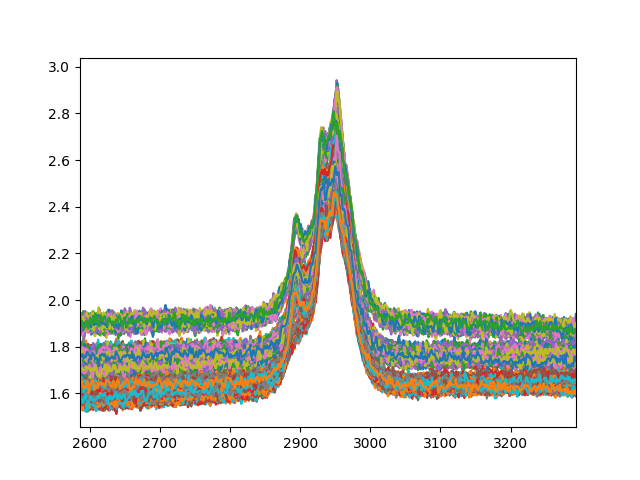
\includegraphics[width=\textwidth]{sdrawsp1.png}
  \caption{\label{spectrum2} Zoomed section of the stacked raw spectra of ngc5291 made with {\tt sdrawsp}.
    Even without any calibration the signal is clearly visible. However, it's not ngc5291, it's ngc0000.
    You will later see the galaxy is near channel 16000, in the middle of the spectrum.}
\end{figure}


\subsection{Case study 1: ngc5291}

Lets start with GBTIDL:

\begin{lstlisting}

GBTIDL -> filein, 'ngc5291.fits' 
GBTIDL -> summary
  Scan           Source      Vel    Proc Seq    RestF nIF nInt nFd     Az    El
-------------------------------------------------------------------------------
    51          NGC5291   4386.0   OnOff   1    1.420   1   11   1  198.2  18.8
    52          NGC5291   4386.0   OnOff   2    1.420   1   11   1  198.7  18.9
    53          NGC5291   4386.0   OnOff   1    1.420   1   11   1  199.1  18.5
    54          NGC5291   4386.0   OnOff   2    1.420   1   11   1  199.7  18.6
    55          NGC5291   4386.0   OnOff   1    1.420   1   11   1  200.1  18.2
    56          NGC5291   4386.0   OnOff   2    1.420   1   11   1  200.7  18.3
    57          NGC5291   4386.0   OnOff   1    1.420   1   11   1  202.1  17.5
    58          NGC5291   4386.0   OnOff   2    1.420   1   11   1  202.7  17.6
\end{lstlisting}

So the user sees 8 scans, but they come in pairs as defined by ``Seq'' (PROCSEQN).  The
PS calibration is done with the {\tt getps} command. They come in pairs, so we only
loop over 4 ``odd'' scans (``even'' scans would produce exactly the same result).
{\tt plnum} refers the XX and YY polarization, which for PS data are hidden in the SAMPLER
meta data.

\begin{lstlisting}
GBTIDL -> for i=51,57,2 do begin getps, i, plnum=0 & accum & end  
Scan:    51 (IF:0 FD:0 PL:0)   units: Ta (K)  Tsys:  19.35    19.73
Scan:    53 (IF:0 FD:0 PL:0)   units: Ta (K)  Tsys:  19.42    19.73
Scan:    55 (IF:0 FD:0 PL:0)   units: Ta (K)  Tsys:  19.48    19.86
Scan:    57 (IF:0 FD:0 PL:0)   units: Ta (K)  Tsys:  19.83    20.06

GBTIDL -> for i=51,57,2 do begin getps, i, plnum=1 & accum & end  
Scan:    51 (IF:0 FD:0 PL:1)   units: Ta (K)  Tsys:  19.49    19.89
Scan:    53 (IF:0 FD:0 PL:1)   units: Ta (K)  Tsys:  19.56    19.92
Scan:    55 (IF:0 FD:0 PL:1)   units: Ta (K)  Tsys:  19.63    20.07
Scan:    57 (IF:0 FD:0 PL:1)   units: Ta (K)  Tsys:  19.98    20.24

GBTIDL -> ave
% ACCUMAVE: Average of :           8 spectra

GBTIDL -> header
--------------------------------------------------------------------------------
Proj: AGBT05B_047_01   Src   : NGC5291                     Obs : Jeff Mangum    

Scan:        51        RADec :  13 47 24.5  -30 24 25     Fsky:   1.399817 GHz
Int :         0        Eqnx  :  2000.0                    Frst:   1.420405 GHz
Pol :         I        V     :  4386.0       OPTI-LSR     BW  :  50.000    MHz
IF  :         0        AzEl  :  198.152      18.772       delF:   1.526    kHz
Feed:         1        Gal   :  317.002      30.931       Exp :  429.7     s
Proc:     OnOff        UT    : +02 05 58.0   2005-06-27   Tcal:    1.45    K
Seqn:         1        LST/HA: +15 07 50.5   1.34         Tsys:   19.59    K
--------------------------------------------------------------------------------

GBTIDL -> write_ascii,'n5291_idl.tab'
\end{lstlisting}

On the screen will now be pretty nice spectrum, that you can zoom in on using
the cursor. See paper fig5 - not placed here yet.

\begin{lstlisting}  
GBTIDL -> list,0,45
 #INDEX           SOURCE       SCAN PROCEDURE POL IFNUM FDNUM        INT SIG CAL
      0          NGC5291         51     OnOff  XX     0     0          0   T   T
      1          NGC5291         51     OnOff  XX     0     0          0   T   F
      2          NGC5291         51     OnOff  XX     0     0          1   T   T
      3          NGC5291         51     OnOff  XX     0     0          1   T   F
      4          NGC5291         51     OnOff  XX     0     0          2   T   T
      5          NGC5291         51     OnOff  XX     0     0          2   T   F
...
     18          NGC5291         51     OnOff  XX     0     0          9   T   T
     19          NGC5291         51     OnOff  XX     0     0          9   T   F
     20          NGC5291         51     OnOff  XX     0     0         10   T   T
     21          NGC5291         51     OnOff  XX     0     0         10   T   F
     
     22          NGC5291         51     OnOff  YY     0     0          0   T   T
     23          NGC5291         51     OnOff  YY     0     0          0   T   F
     24          NGC5291         51     OnOff  YY     0     0          1   T   T
     25          NGC5291         51     OnOff  YY     0     0          1   T   F
...
     41          NGC5291         51     OnOff  YY     0     0          9   T   F
     42          NGC5291         51     OnOff  YY     0     0         10   T   T
     43          NGC5291         51     OnOff  YY     0     0         10   T   F
     44          NGC5291         52     OnOff  XX     0     0          0   T   T
     45          NGC5291         52     OnOff  XX     0     0          0   T   F
\end{lstlisting}

This data has 352 rows in the SDFITS file, organized as follows (see also the GBTIDL
conversation below):  There are 8 scans, each of which has 11 integrations, each of
which has 2 samplers (A9 and A13, which are the XX (-5) and YY (-6) pols), each of which has
two phases of CAL=T and CAL=F. Hence 8 x 11 x 2 x 2 = 352. Another way of writing this in a
5-dimensional array is $DATA(ncal,nint,nsampler,nprocseqn,nscan)$.

Each phase (record) has an DURATION
of 5.0475 secs, but the EXPOSURE varies between 4.81 and 4.91 secs, but mostly bimodal
at about 4.86 and 4.91 secs.  Between each scan there was about a 35 secs pause, the
whole observation took from 2:05:58.00 to 2:28:23.93, about 24 minutes.


Although this {\tt list} command gives a nice summary, it only shows typicall 1/4 of the ``phases'' you will see
in the SDFITS file, skipping over on/off/calon/caloff and pols.
The {\tt gbtoy/bin/sdlist} command will show you all you can possible want. Also note that our command will show you
that the SDFITS file is not always time sorted.


\begin{lstlisting}
  filein, 'ngc5291.fits'
  
  for i=51,57,2 do begin getps, i, plnum=0 & accum & end  
  for i=51,57,2 do begin getps, i, plnum=1 & accum & end
  ave
  stats,6000,12000
  ; -> 0.29487  0.015592  0.24204     0.35086

  write_ascii,'n5291_idl.tab'

  getps, 51, plnum=0
  ; -> Tsys:  19.35    19.73
  stats,6000,12000
  ; -> 0.26267 0.044331 0.11131     0.43709
  accum
  getps, 51, plnum=1
  ; -> Tsys:  19.49    19.89
  accum
  ave
  stats,6000,12000
  ; -> 0.29296 0.031619
  write_ascii,'n5291_51.tab'

  getps, 51, plnum=0, intnum=0
  ; -> Tsys:  19.20    19.96
  stats,6000,12000
  ; -> 0.26469   0.14426 -0.25974     0.81696
  accum
  ; -> 0.26573  0.14347
  getps, 51, plnum=1, intnum=0
  ; -> Tsys:  19.30    20.08
  accum
  ave
  stats,6000,12000
  ; -> 0.28946 0.10193
  write_ascii,'n5291_51a.tab'

  getrec,0
  stats,6000,12000
  ; -> 1.2461      0.13825  1.0871      1.5781
  write_ascii,'n5291_0.tab'
  
  getrec,1
  stats,6000,12000  
  ; -> 1.1596      0.12798  1.0093      1.4739
  write_ascii,'n5291_1.tab'
  
  getrec,44
  stats,6000,12000  
  ; -> 1.2280      0.13591  1.0713      1.5567
  write_ascii,'n5291_44.tab'

  getrec,45
  stats,6000,12000  
  ; -> 1.1394      0.12588  0.99495      1.4452
  write_ascii,'n5291_45.tab'
  
  
\end{lstlisting}






In figure \ref{waterfall} we show the result of running {\tt sdimage}, which creates a 2D image ``Waterfall Plot''
with channels along X and time along Y. The CARTA program in particular can also be a good diagnostic to look at the data quality.
The ordering of the  different ``phases'' that go into an ``integration'' for a ``scan'' can be easily seen
in this way of viewing the data.

\begin{figure}[h]
\centering
  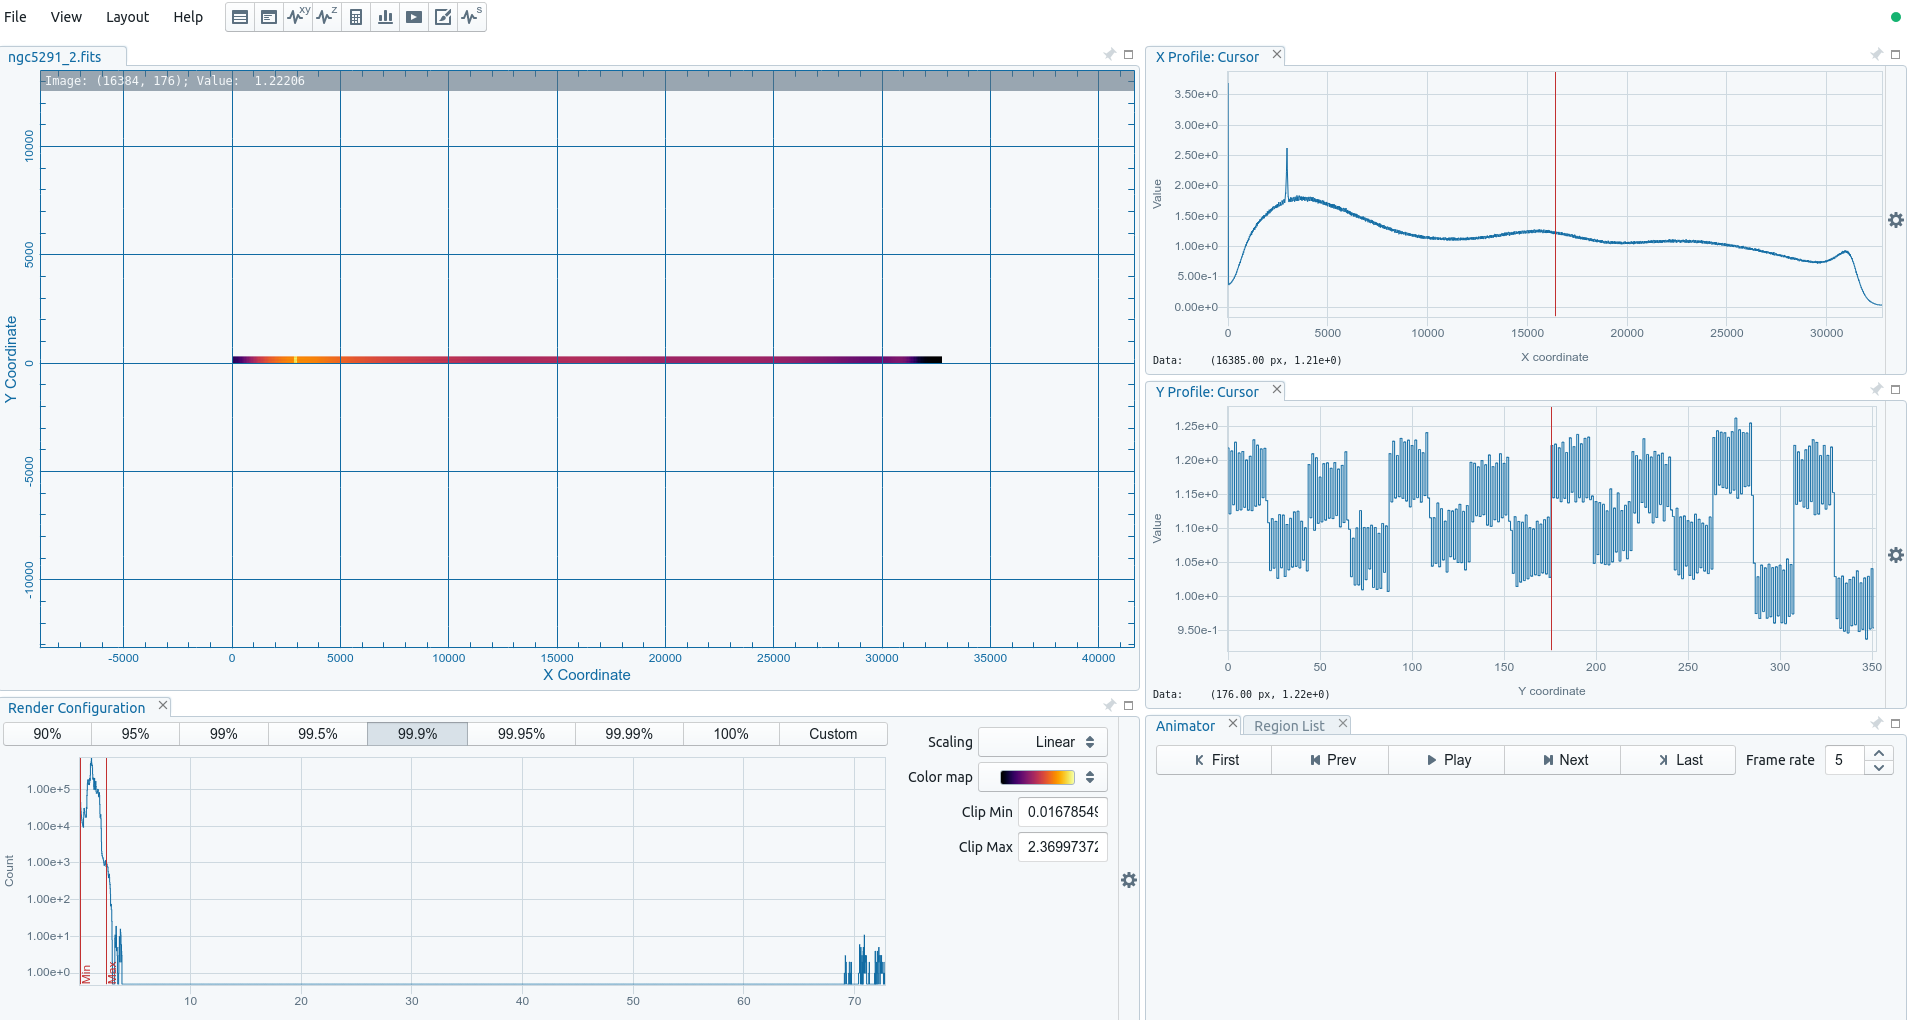
\includegraphics[width=\textwidth]{ngc5291_2a.png}
  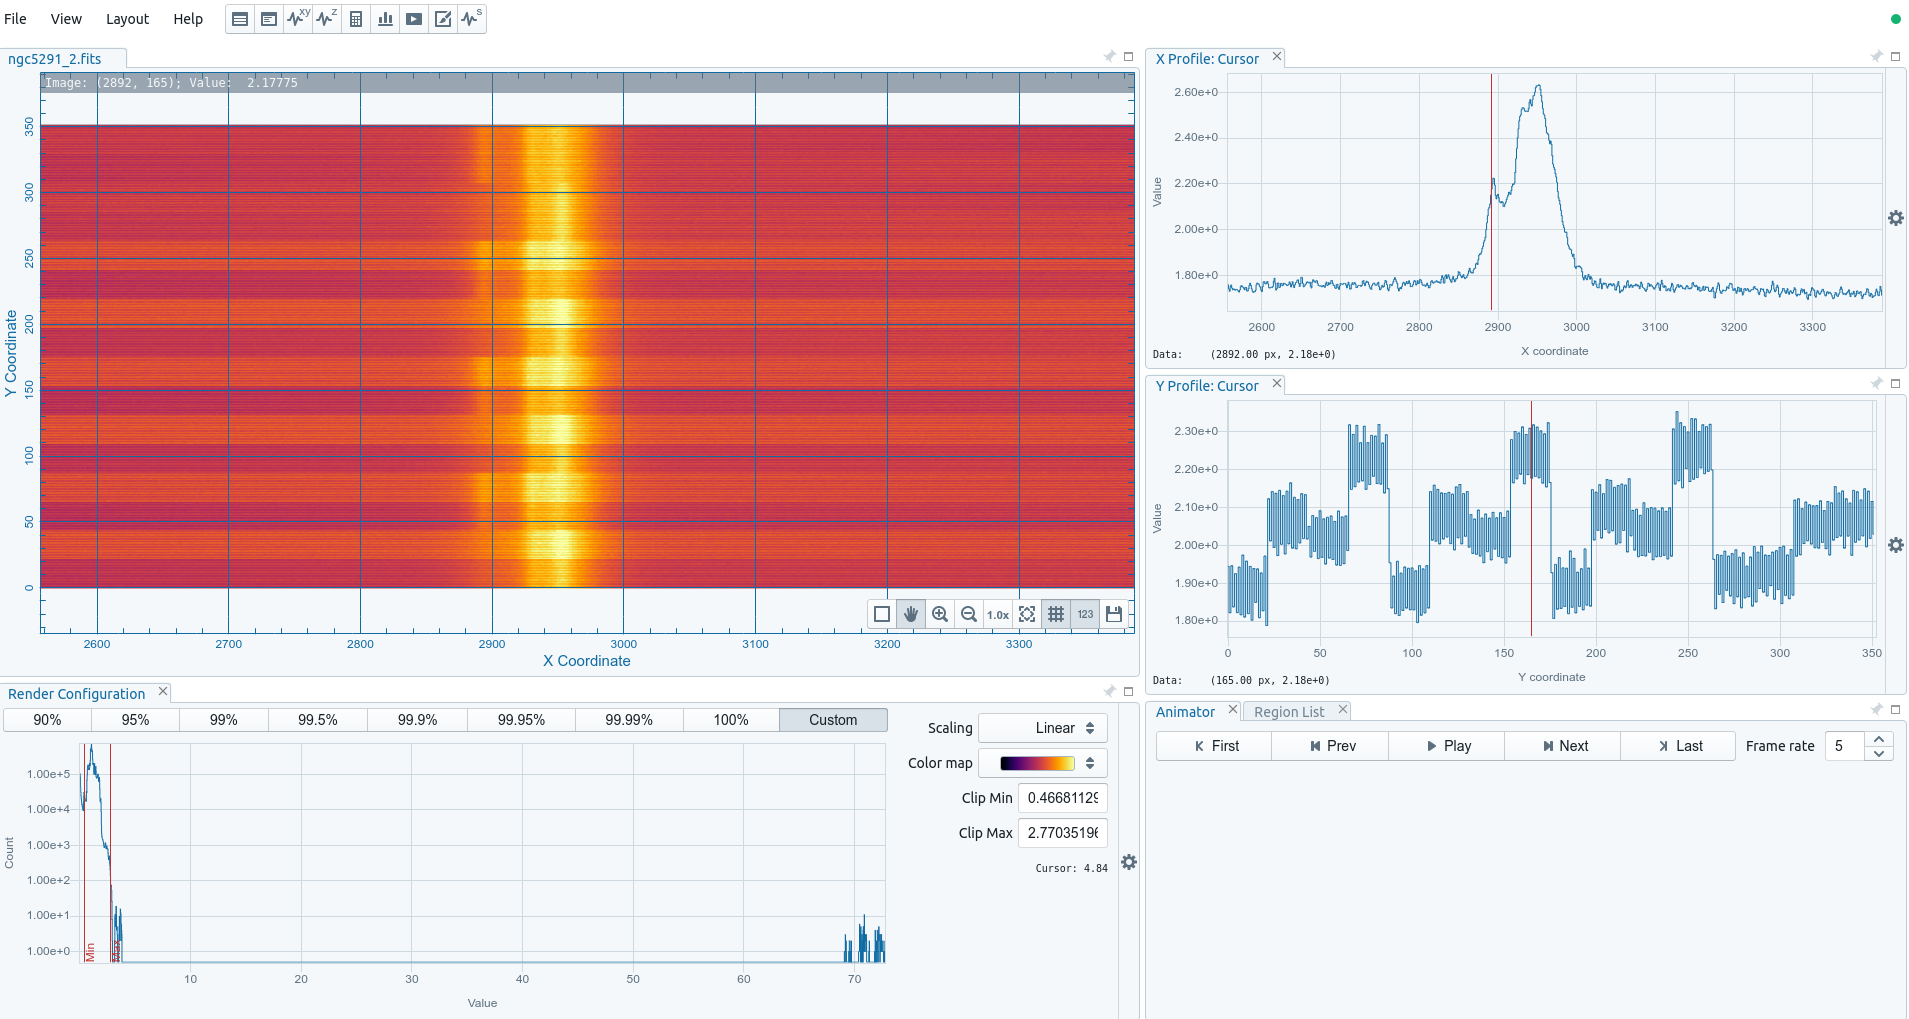
\includegraphics[width=\textwidth]{ngc5291_2b.png}
  \caption{\label{waterfall} Viewing an sdimage version of ngc5291 with CARTA:
    full view and zoomed version on the HI spectral line. This kind
    of image is also known as a {\bf Waterfall Plot}. Channels run along X, time/sequence along Y.
    Compare this to figure \ref{bintable}.}
\end{figure}

\subsection{Low Level GBTIDL}

In order to reproduce this example, we need to consider the following calibration procedure:
$$
T_A = T_{sys} { { (ON-OFF)} \over {ON} }
$$



\section{Software}

The following software has been discussed in this paper (where available, we use their ASCL id for reference):


\begin{enumerate}
\item UniPOPS: \url{https://ascl.net/1503.007}
\item DISH (within AIPS++) - not supported anymore
\item GBTIDL: \url{https://ascl.net/1303.019}
\item comb: \url{https://ascl.net/code/v/2397}   (submitted)
\item CLASS (within GILDAS) \url{https://ascl.net/1305.010}
\item pyspeckit: \url{https://ascl.net/1109.001}
\item aoflagger: \url{https://ascl.net/1010.017}
\item CASA \url{https://ascl.net/1107.013}
\item specutils: \url{https://ascl.net/1902.012}
\item specreduce:  \url{https://github.com/astropy/specreduce}
\item specviz: \url{https://ascl.net/1902.011}
\item spectral-cube (within radio-astro-tools) \url{https://ascl.net/1609.017}
\item Astropy \url{https://ascl.net/1304.002}
\item SpecViz \url{https://ascl.net/1902.011}
\item gbt-pipeline \url{https://github.com/GreenBankObservatory/gbt-pipeline}
\item gbtgridder \url{https://github.com/GreenBankObservatory/gbtgridder}
\item gbtpipe \url{https://github.com/GBTSpectroscopy/gbtpipe}
\item AIPS \url{https://ascl.net/9911.003}
\item ParselTongue \url{https://ascl.net/1208.020}
\item SpecX \url{https://ascl.net/1310.008}
\item NOD3 \url{https://ascl.net/1711.024}

\end{enumerate}

\bibliographystyle{unsrt}
\bibliography{gbtoy}

\newpage
\section*{Appendix A: work}

Here is summary of the initial work packages and deliverables for the first 3 months.
\subsection{Work packages}

1) Survey current python codes (pyspeckit, specutils)

2) Survey current SD packages for functionality (comb, CLASS, NOD3, casa)

3) Design Document

\subsection{Deliverables}

1) Results of WP1 and WP2 in a white paper [early Dec 2019]

2) Design Document with two use cases (PS,FS) for a PDR with GBO.

\section*{Appendix B: codes}

The following samplings of code and scripts you may now find scatterred in {\tt gbtoy}:
\footnote{\url{https://github.com/teuben/gbtoy}}

\begin{itemize}
  \item {\tt bin/sdheader}:  list the header and some size info
  \item {\tt bin/sdimage}:    convert spectra into a 2D image (nchan x nrows). Creates {\tt basename\_2.fits}
  \item {\tt bin/sdinspect}:  plot a spectrum using pyspeckit
  \item {\tt bin/sdlist}:  list all the FIELDS or the content of a single FIELD
  \item {\tt gbtidl.py}: peter's cross atlantic coding sprint, uses pyspeckit (POC, unfinished of course)
\end{itemize}       

\section*{Appendix C: benchmarks}

Two datasets have come out that are useful for benchmarking:

\subsection{ngc5271.fits}

This is the PS data Example 1 in the GBTIDL manual. ``easy'' to understand. Raw data. 352 rows.  Used with a simple {\tt filein} command.

\subsection{EDGE NGC2347}

This is more the new style, many files in a directory. We have 6 files totalling 2GB. Used with the more complex {\tt dirin} command.
Tony Wong has provided an IDL script that might help, but so far this has been more useful to check the I/O speed and on the question
for the need for an index file.




\end{document}
